\documentclass[a4paper]{article}

\setlength{\parindent}{0pt}
\setlength{\parskip}{1em}

\pagestyle{headings}

\usepackage{amssymb}
\usepackage{amsmath}
\usepackage{amsthm}
\usepackage{mathtools}
\usepackage{graphicx}
\usepackage{hyperref}
\usepackage{color}
\usepackage{microtype}
\usepackage{tikz}
\usepackage{pgfplots}
\usepackage{pgfplotstable}

\newcommand{\N}{\mathbb{N}}
\newcommand{\Q}{\mathbb{Q}}
\newcommand{\Z}{\mathbb{Z}}
\newcommand{\R}{\mathbb{R}}
\newcommand{\C}{\mathbb{C}}
\newcommand{\D}{\mathcal{D}}
\renewcommand{\S}{\mathcal{S}}
\renewcommand{\P}{\mathbb{P}}
\newcommand{\F}{\mathbb{F}}
\newcommand{\E}{\mathbb{E}}
\newcommand{\bra}{\langle}
\newcommand{\ket}{\rangle}


\graphicspath{{Image/}}

\hypersetup{
    colorlinks=true,
    linktoc=all,
    linkcolor=blue
}

\theoremstyle{definition}
\newtheorem*{axiom}{Axiom}
\newtheorem*{claim}{Claim}
\newtheorem*{conv}{Convention}
\newtheorem*{coro}{Corollary}
\newtheorem*{defi}{Definition}
\newtheorem*{eg}{Example}
\newtheorem*{lemma}{Lemma}
\newtheorem*{notation}{Notation}
\newtheorem*{prob}{Problem}
\newtheorem*{post}{Postulate}
\newtheorem*{prop}{Proposition}
\newtheorem*{rem}{Remark}
\newtheorem*{thm}{Theorem}

\DeclareMathOperator{\vdiv}{div}
\DeclareMathOperator{\grad}{grad}
\DeclareMathOperator{\curl}{curl}
\DeclareMathOperator{\Ann}{Ann}
\DeclareMathOperator{\Fit}{Fit}
\DeclareMathOperator{\Diag}{Diag}
\DeclareMathOperator{\tr}{tr}
\DeclareMathOperator{\im}{im}
\DeclareMathOperator{\Mat}{Mat}
\DeclareMathOperator{\Log}{Log}
\DeclareMathOperator{\Isom}{Isom}
\DeclareMathOperator{\Mesh}{Mesh}
\DeclareMathOperator{\Sym}{Sym}
\DeclareMathOperator{\Aut}{Aut}
\DeclareMathOperator{\cosech}{cosech}
\DeclareMathOperator{\Card}{Card}
\DeclareMathOperator{\Gal}{Gal}


\setcounter{section}{-1}

\begin{document}

\title{Coding and Cryptography}

\maketitle

\newpage

\tableofcontents

\newpage

\section{Miscellaneous}

132

\newpage

\section{Introduction to communication channels and coding}
For example, given a message $M = "Call me!"$ which we wish to send by email. We first encode t as binary strings using ASCII. So $f(C) = 1000011$, $f(a) = 1100001$, $f^*(M) = 1000011 1100001 ... 0100001$. 

The message goes from the source to the receiver after encoded by the source and decoded by the receiver via a channel, where errors could occur. The basic problem is, given a source and a channel (described probabilistically, we aim to design an encoder and a decoder in order to transmit information economically, reliably, and preserving privacy (secretly).

Some examples of each aspect:\\
\emph{economcically}: Morse code, where common letters have shorter codewords;\\
\emph{reliability}: every book has an ISBN of form $a_1...a_{10}$ where $a_i \in \{0,1,...,9\}$ for $1 \leq i \leq 9$ and $a_{10} \in \{0,1,...,9,X\}$, s.t. $10 a_1 + 9a_2+...+a_{10} \equiv 0 \pmod 11$, where we treat $X$ as 10. In this way errors can be detected, although not corrected. There is another version of ISBN which is 13 digit;\\
\emph{preserve privacy} RSA.

A communication channel takes letters from an input alphabet $\Sigma_1 = \{a_1,...,a_r\}$ and emits letters from an output alphabet $\Sigma_2 = \{b_1,...,b_s\}$.

A channel is determined by the probabilities $P(y_1,...,y_k$ received$|x_1,...,x_k$ sent$)$.

\begin{defi}
A \emph{discrete memoryless channel}(DMC) s a channel for which $P_{ij} = P(b_j$ received$|a_i$ sent$)$ is the same each time the channel is used, and is independent of all past and future. The channel matrix is the $r \times s$ matrix with entrices $p_{ij}$. Note the rows sum to $1$.
\end{defi}

\begin{eg} (Binary Symmetric Channel, BSC)\\
BSC has $\Sigma_1 = \Sigma_2 = \{0,1\}$, $0 \leq p \leq 1$. It has channel matrix ${{1-p \ p} \choose {p \ 1-p}}$, i.e. $p$ is the probability symbol is mistransmitted.
\end{eg}

\begin{eg} (Binary Erasure Channel)\\
$\Sigma_1 = \{0,1\}$, $\Sigma_2 = \{0,1,*\}$, $0 \leq p \leq 1$. Then the channel matrix is ${{1-p \ p \ 0} \choose {0 \ p \ 1-p}}$, i.e. $p$ is the probability that a synbol can't be read.
\end{eg}

Informal definition: A channel's capacity is the highest rate at which information can be reliably transimitted over the channel. Here rate means the units of information per unit tme (we want that high), and reliably means arbitrarily small error probability.

There are 3 sections:\\
1) Noiseless coding (data compression);\\
2) Error control codes;\\
3) Cryptography.

\subsection{Noiseless coding}
\begin{notation}
For $\Sigma$ an alphabet that $\Sigma^* = \bigcup_{n \geq 0} \Sigma^n$ be th set of all finite strings of elements of $\Sigma$.
\end{notation}

If $x=x_1...x_r$, $y=y_1...y_s$ are strings from $\Sigma$, write $xy$ for the concatenation $x_1...x_ry_1...y_s$. Further, $|x_1...x_ry_1...y_s| = r+s$ the length of string.

\begin{defi}
Let $\Sigma_1,\Sigma_2$ be two alphabets. A \emph{code} is a function $f:\Sigma_1 \to \Sigma_2^*$. The strings $f(x)$ for $x \in E$ are called \emph{codewords}.
\end{defi}

\begin{eg} (Greek five code)\\
$\Sigma_1 = \{\alpha,\beta,...,\omega\}$ (24 letters); $\Sigma_2 = \{1,2,3,4,5\}$ (more used). Now let $\alpha \to 11, \beta \to 12, ...,\omega \to 54$.
\end{eg}

\begin{eg}
$\Sigma_1 = \{$all words in the dictionary$\}$. =,$\Sigma_2 = \{A,B,...,space\}$. Then $f=$'spell the word and a space.'
\end{eg}

We sent a message $x_1,...,x_n \in \Sigma^*_1$ as $f(x_1)f(x_2)...f(x_n) \in \Sigma_2^*$, i.e. extend $f$ to $f^* : \Sigma_1^* \to \Sigma_2^*$.

\begin{defi}
A code $f$ is \emph{decipherable} if $f^*$ is injective, i.e. every string from $\Sigma_2$ arises from at most one message.
\end{defi}

Note that $f$ being injective is not enough. See this example:

\begin{eg}
$\Sigma_1 = \{1,2,3,4\}$, $\Sigma_2 = \{0,1\}$, $f(1) = 0$, $f(2) = 1$, $f(3) = 00$, $f(4) = 01$. Then $f$ is injective, but $f^*(312) = 0001 = f^*(114)$ so $f^*$ is not decipherable.
\end{eg}

\begin{notation}
If $|\Sigma_1| = m$, $|\Sigma_2| = a$, then we say $f$ is an $a$-ary code of size $m$ (in particular, if $a=2$ we use the word binary).
\end{notation}

Our aim is to construct decipherable codes with short word lengths.

Provided $f:\Sigma_1 \to \Sigma^*_2$ is injective, the following codes are always decipherable:\\
(1) A \emph{Block code} is a code with all codewords of the same length (eg Greek fire code);\\
(2) In a \emph{comma code} we reserve one letter from $\Sigma_2$ that is only used to signal the end of the codeword (example 2);\\
(3) A \emph{prefix-free} code is a code where no codeword is a prefix of another (If $x,y \in \Sigma^*_2$, $x$ is a prefix of $y$ if $y=xz$ for some $z \in \Sigma^*_2$).

\begin{rem}
(1) and (2) are special cases of (3).
\end{rem}

Prefix-free codes are also known as \emph{instantaneous codes} (i.e. a word can be recognised as soon as its complete), or \emph{self-punctuating codes}.

\begin{thm} (1.1, Kraft's inequality)\\
Let $\Sigma_1| = m$, $\Sigma_2| = a$. A prefix-free code $f:\Sigma_1 \to \Sigma_2^*$ with word lengths $s_1,...,s_m$ exist iff $$\sum_{i=1}^m a^{-s_i} \leq 1$$
\begin{proof}
First we prove forward implication. Consider an infinite tree where each has a descendents, labelled by the elements of $\Sigma_2$. Each codeword corresponds to a node, the path from the root to this node spelling at the codeword. Assuming $f$ is prefix-free, no codeword is the ancestor of any other. Now view the tree as a network with water being pumped in at constant rate and divding the flow equally at each node. The total amount of water we can extract at the codewords is $\sum_{i=1}^m a^{-s_i}$ which is therefore $\leq 1$.

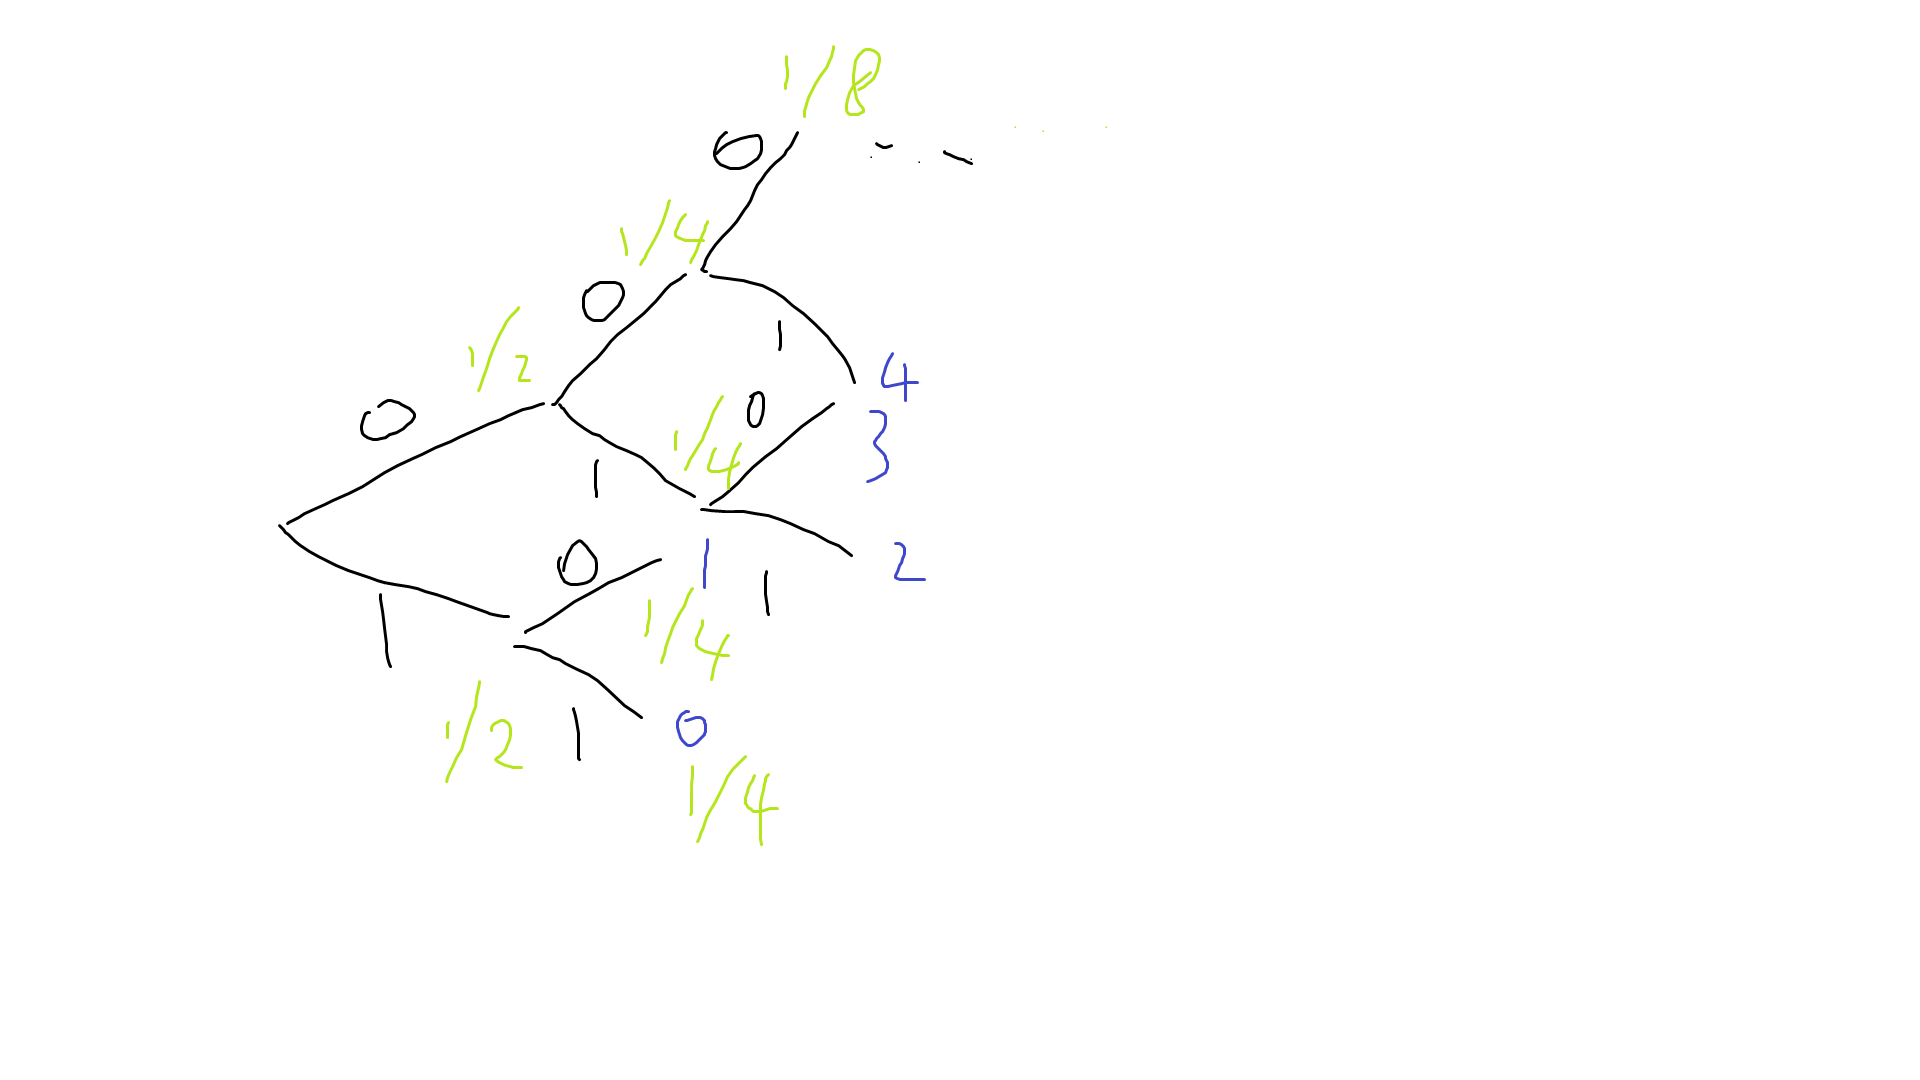
\includegraphics[scale=0.5]{image/CC_01.png}

Conversely, suppose we can construct a prefix-free code with word lengths $s_1,...,s_m$ , wlog $s_1 \leq s_2 \leq ... \leq s_m$. We pick codewords of lengths $s_1,...,$ sequentially ensuring previous codewords are not prefixes. Suppose there is no valid choice for the $r^{th}$ codeword. The constructing the tree as above gives $\sum_{i=1}^{r-1} a^{-s_i} = 1$, contradicting our assumption. So we can construct a prefix-free code.
\end{proof}
\end{thm}

\begin{thm} (1.2, Mcmillan)\\
Every decipherable code satisfies Kraft's inequality.
\begin{proof} (Karush)\\
Let $f:\Sigma_1 \to \Sigma_2^*$ be a decipherable code with word lengths $s_1,...,s_m$, let $s = \max_{1 \leq i \leq m} s_i$. Let $r \in \N$, $$(\sum_{i=1}^m a^{-s_i})^r = \sum_{b = 1}^{rs} b_i a^{-l}$$ where $b_i$ is the number of ways of choosing $r$ codewords of toatl length $l$. $f$ decipherable implies that $b_l \leq |\Sigma_2|^l = a^l$. Thus $(\sum_{i=1}^m a^{-s_i})^r \leq \sum_{l=1}^{rs} a^l a^{-l} = rs$, so $\sum_{i=1}^m a^{-s_i} \leq (rs^{1/r}) \to 1$ as $r \to \infty$. So $\sum_{i=1}^m a^{-s_i} \leq 1$.
\end{proof}
\end{thm}

So we have a corollary: a decipherable code with prescribed word lengths exist iff there exists a prefix-free code with the same word lengths.

So we can restrict our attention to prefix-free codes.

\subsection{Mathematical entropy}
Entropy is a measure of 'randomness' or 'certainty'. Consider a random variable $X$ taking values $x_1,...,x_n$ with probability $p_1,...,p_n$ ($\sum p_i = 1$, $0 \leq p_i \leq 1$). The entropy $H(x)$ is roughly speaking the expected number of tosses of a fair coin needed to simulate $X$ (or the expected number of yes/no questions we need to ask in order to establish the value of $X$).

\begin{eg}
Suppose $p_1 = p_2 = p_3 = p_4 = \frac{1}{4}$. We identify $\{x_1,...,x_4\}$ with $\{HH,HT,TH,TT\}$, so $H(x) = 2$.
\end{eg}

\begin{eg}
$(p_1,p_2,p_3,p_4) = (1/2,1/4,1/8,1/8)$. Then $H(x) = 1/2+1/4 \times 2 + 1/8 \times 3 + 1/8 \times 3=7/4$. So the entropy here is smaller.

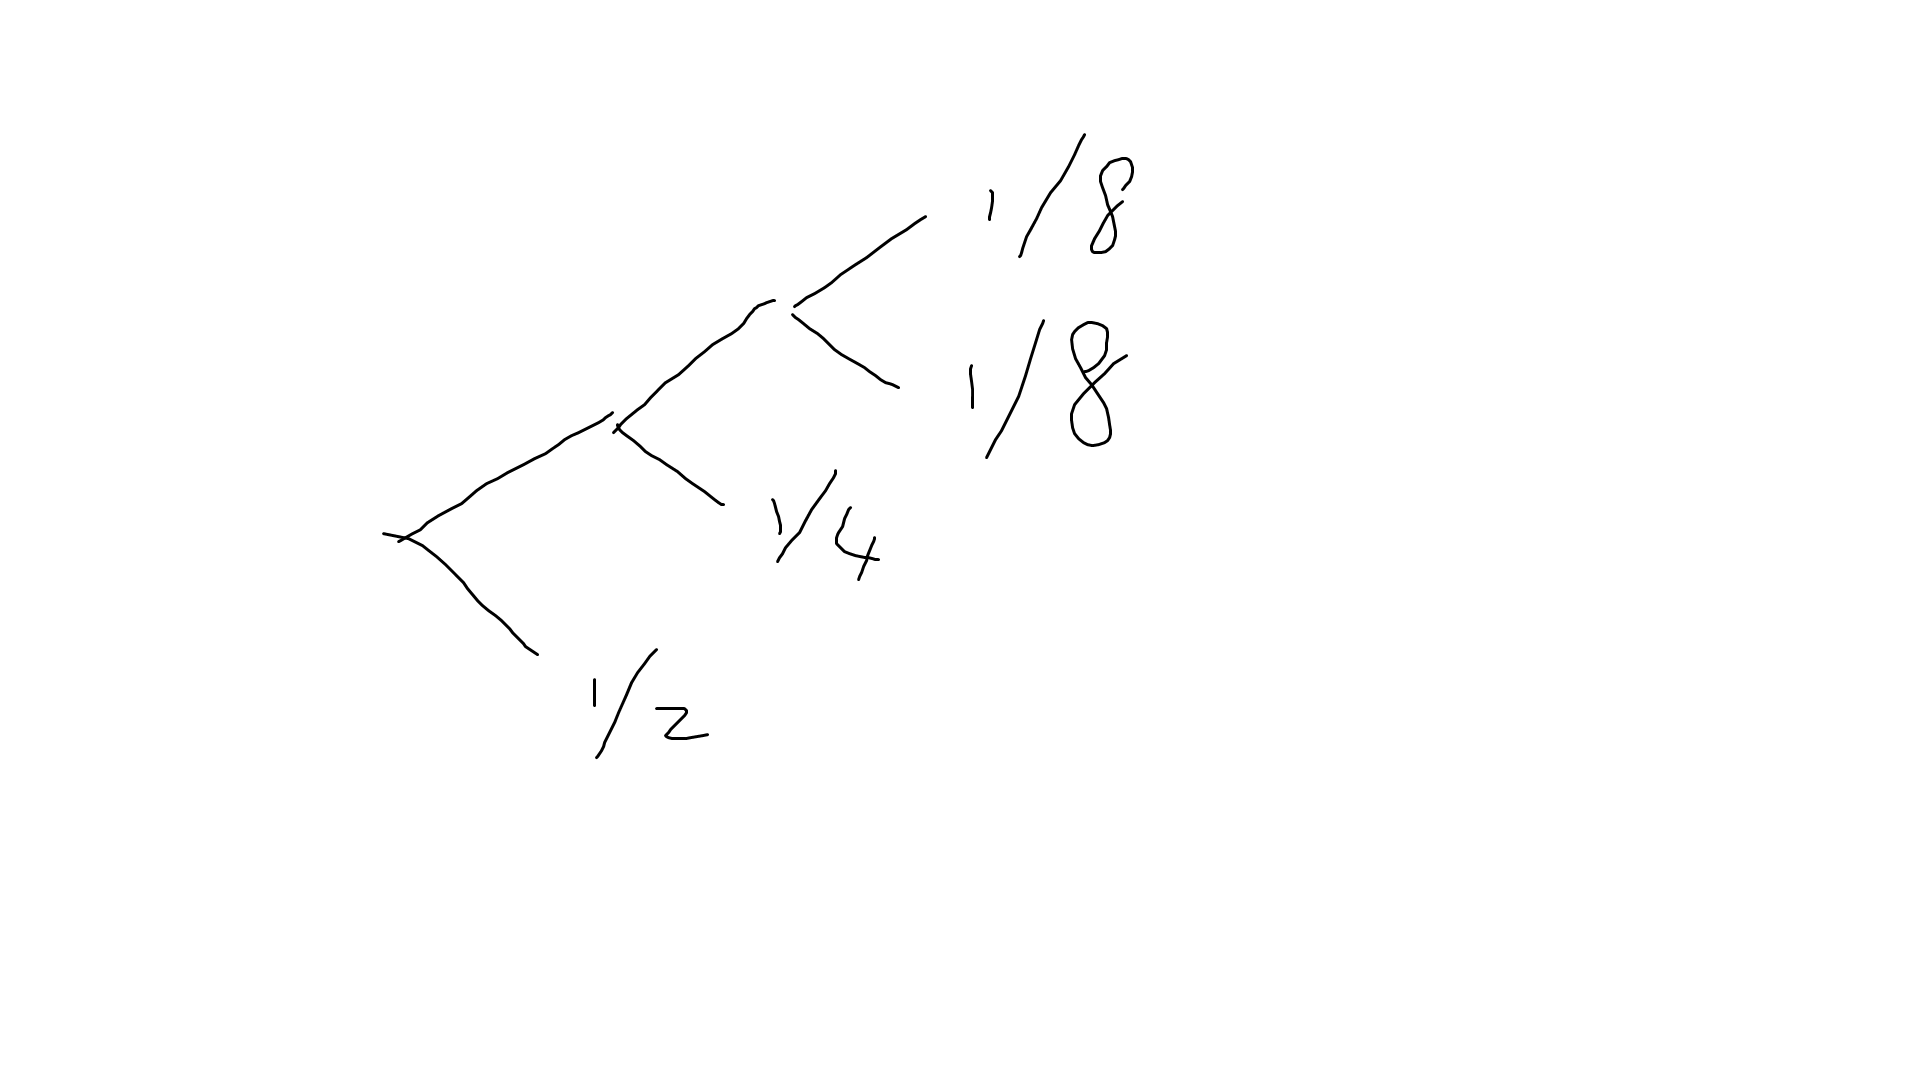
\includegraphics[scale=0.5]{image/CC_02.png}
\end{eg}

So in some sense, there is more randomness in the first example than the second.

\begin{defi} (Entropy)\\
The entropy of $X$, $$H(X) = H(p_1,...,p_n) = -\sum_{i=1}^n p_i \log p_i$$ where, as most of the time in this course, $\log = \log_2$.
\end{defi}

\begin{rem}
(1) If $p_i = 0$, we define $p_i \log p_i = 0$;\\
(2) $H(X) \geq 0$.
\end{rem}

\begin{eg} (3)\\
We toss a biased coin with $\P($heads$) = p$. Write $H(p) = H(p,1-p) = -p\log p - (1-p)\log(1-p)$. If $p=0$ or $1$, the outcome is certain and so entropy is $0$. Entropy is maximal where $p=1/2$ (check), a fair coin.

Note the entropy can also be viewed as the expected value of the information of $X$, where information is given by $I(X=x) = -\log \P(X=x)$. For example, if a coin always lands heads, we gain on information from tossing the coin.\\
This entropy is the average amount of information conveyed by a random variable $X$.
\end{eg}

\begin{lemma} (1.3, Gibbs' inequality)\\
Let $p_1,...,p_n$ and $q_1,...,q_n$ be probability distributions. Then $-\sum p_i \log p_i \leq -\sum p_i \log q_i$, with equality iff $p_i = q_i$.
\begin{proof}
It supplies to prove the inequality with $\log$ replaced by $\ln$. Note $\ln x \leq x-1$ with equality iff $x=1$. Let $I = \{1 \leq i \leq n: p_i \neq 0\}$. Then $\ln \frac{q_i}{p_i} \leq \frac{q_i}{p_i}-1$ $\forall i \in I$. So $\sum_{i \in I} p_i \ln \frac{q_i}{p_i} \leq \sum q_i - \underbrace{\sum p_i}_{=1} \leq 0$. Rearranging we get $-\sum_{i \in I} p_i \ln p_i \leq -\sum_{i \in I} p_i \ln q_i$, so $-\sum_{i=1}^n p_i \ln p_i \leq -\sum_{i=1}^n p_i \ln q_i$. If equality holds then $\frac{q_i}{p_i} = 1$ $\forall i \in I$, so $\sum_{i \in I} q_i = 1$ $\implies p_i = q_i$ for $1 \leq i \leq n$.
\end{proof}
\end{lemma}

\begin{coro}
$H(p_1,...,p_n) \leq \log n$ with equality iff $p_1 = p_2 = ... = p_n =\frac{1}{n}$.
\begin{proof}
Take $q_1=q_2=...=q_n = \frac{1}{n}$ in previous lemma.
\end{proof}
\end{coro}

Two alphabets $\Sigma_1,\Sigma_2$ with $|\Sigma_1| =m$, $|\Sigma_2| = a$ ($m \geq 2, a \geq 2$). We model the source as a sequence of random variables $X_1,X_2,...$ taking values in $\Sigma_1$.

\begin{defi}
A \emph{Bernoulli} or \emph{memoryless} source is a sequence of independently, identically distributed random variables, i.e. for each $\mu \in \Sigma_i$, the probability of $X_i = \mu$ is independent of $i$ and independent of all past and future symbols emitted. Thus $$\P(X_1=x_1,...,X_k = x_k) = \prod_{i=1}^k \P(X_i = x_i)$$

Let $\Sigma_1 =\{\mu_1,...,\mu_n\}$, $p_i = \P(X =\mu_i)$ and assume $p_i > 0$. The \emph{expected word length} of a code $f:\Sigma_1 \to \Sigma^*_2$ with word lengths $s_1,...,s_m$ is $E(S) = \sum_{i=1}^m p_i s_i$.
\end{defi}

\begin{defi}
A code $f:\Sigma_1 \to \Sigma^*_2$ is \emph{optimal} if it has the shortest possible expected word length among decipherable code.
\end{defi}

\begin{thm} (1.4, Shannon's Noiseless Coding theorem)\\
The minimum expected word length of a decipherable code $f:\Sigma_1\to \Sigma^*_2$ satisfies $$\frac{H(x)}{\log a} \leq E(S) < \frac{H(X)}{\log a} + 1$$
\begin{proof}
The lower bound is given by combining Gibbs and Kraft inequalities. Let $q_i = \frac{a^{-s_i}}{c}$ where $c = \sum a^{-s_i} \leq 1$ by Kraft's inequality. Note $\sum q_i = 1$. Now 
\begin{equation*}
\begin{aligned}
H(X) = -\sum p_i \log p_i &\leq -\sum_i p_i \log q_i \\
&= \sum_i p_i (s_i \log a + \log c)\\
&= (\sum_i p_i s_i) \log a + \log c\\
&\leq E(s) \log a
\end{aligned}
\end{equation*}
We get equality if and only if $p_i = a^{-s_i}$ for some integers $s_i$.

For the upper bound, put $s_i = \lceil -\log_a p_i \rceil$. We have $\log_a p_i \leq s_i < -\log_a p_i +1$, so $a^{-s_i} \leq p_i \implies \sum a^{-s_i} \leq \sum p_i \leq 1$. So by theorem (1.), there exists a prefix-free code with word lengths $s_1,...,s_m$.\\
Also,
\begin{equation*}
\begin{aligned}
E(S) &= \sum p_i s_i\\
&< \sum p_i (-\log_a p_i + 1)\\
&= \frac{H(X)}{\log a} + 1
\end{aligned}
\end{equation*}
\end{proof}
\end{thm}

\begin{rem}
The lower bound holds for all decipherable codes.
\end{rem}

Shannon-Fano Coding (as in Goldie $\&$ Pinch):\\
This follows from the proof above. Set $s_i = \lceil -\log_a p_i\rceil$ and construct a prefix-free code with word lengths $s_1,...,s_m$ by taking the $s_i$ in increasing order ensuring that previous codewords are not prefixes. The Kraft inequality ensures there is enough room.

\begin{eg}
$\mu_1,...,\mu_5$ emitted with probabilities $0.4,0.2,0.2,0.1,0.1$. We try to construct Shannon-Famo code (with $a=2$, $\Sigma_2 = \{0,1\}$):
\begin{equation*}
\begin{aligned}
\begin{matrix}
p_i & \lceil -\log p_i\rceil & \text{code}\\
0.4 & 2 & 00\\
0.2 & 3 & 010\\
0.2 & 3 & 100\\
0.1 & 4 & 1100\\
0.1 & 4 & 1110
\end{matrix}
\end{aligned}
\end{equation*}
The expected word length is $2 \times 0.4 + 3 \times 0.2 + 3 \times 0.2 + 4 \times 0.1 + 4 \times 0.1 = 2.8$.\\
As a comparison, $H(X) \approx 2.12$, which is consistent with our previous inequality.
\end{eg}

\begin{defi} (Huffman coding)\\
For simplicity we take $a=2$. Let $\Sigma_1 = \{\mu_1,...,\mu_m\}$, $p_i = \P(X=\mu_i)$. WLOG $p_1 \geq p_2 \geq ... \geq p_m$.  Huffman coding is defined inductively:\\
If $m=2$, assign codewords $0$ and $1$;\\
If $m>2$, find a Huffman coding in the case of meesages $\mu_1,\mu_2,...,\nu$ with probaiblities $p_1,p_2,...,p_{m-1}+p_m$; append $0$ (1 respectively) to the codeword for $\nu$ tove a codeword for $\mu_{m-1}$ ($\mu_m$ respectively).
\end{defi}

\begin{rem}
(i) This construction gives a prefix-free code;\\
(ii) We exercise some choice when some of the $p_i$ are equal. So Huffman codes are not unique.
\end{rem}

\begin{eg}
We look at the previous example:

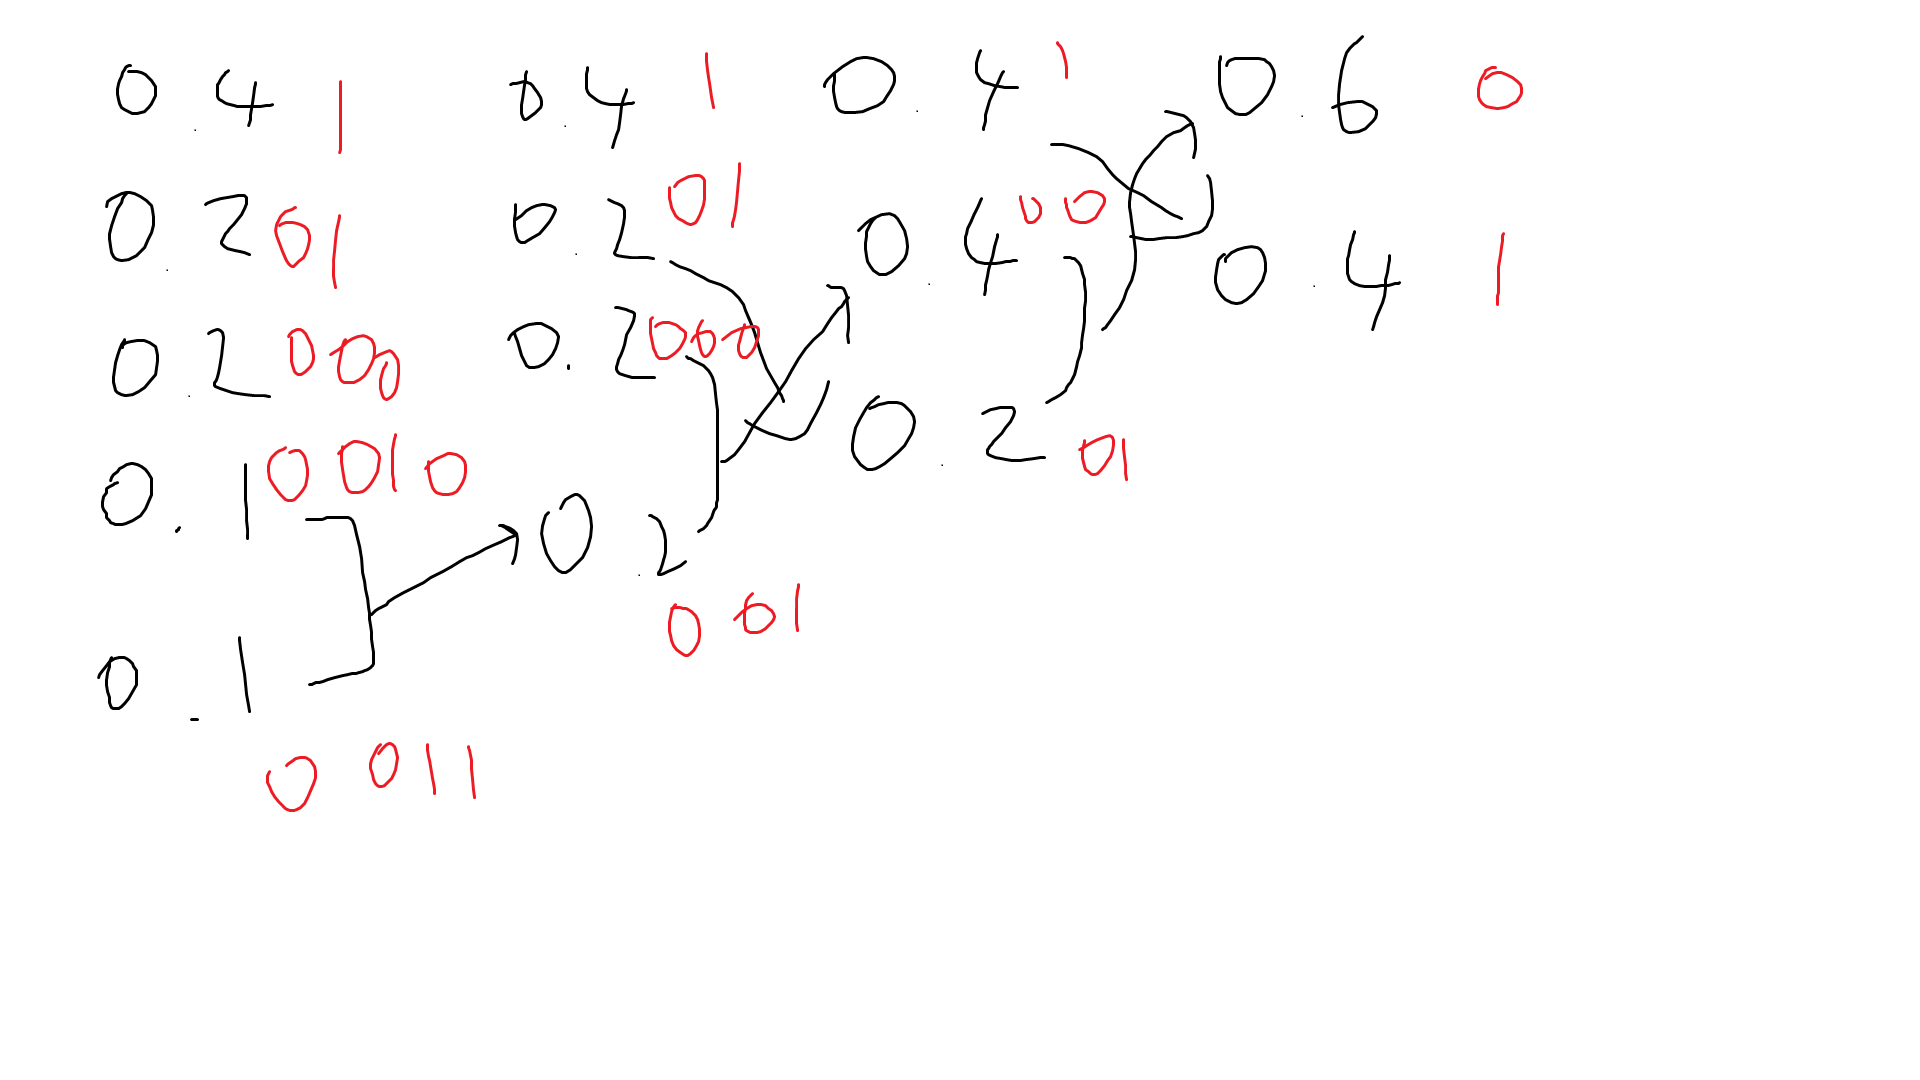
\includegraphics[scale=0.6]{image/CC_03.png}

So we get $\{1,01,000,0010,0011\}$ as the prefix-free code constructed. The expected word length is $2.$, which is better then the Shannon-Fano coding.
\end{eg}

\begin{thm} (1.5)\\
Huffman coding is optimal.
\end{thm}

\begin{lemma} (1.6) \\
Suppose $\mu_1,...,\mu_m \in \Sigma_1$ emitted with probabilities $p_1,...,p_m$. Let $f$ be an optimal prefix-free code with word lengths $s_1,...,s_m$. Then\\
(i) if $p_i > p_j$, then $s_i \leq s_j$;\\
(ii) there exists 2 codewords of maximal length which are equal up to the last digit.\\
\begin{proof}
(i) Otherwise, swap codewords $i$ and $j$ to reduce the expected word length.\\
(ii) If not, then either there is only one codeword of maximal length, or any two codewords of maximal length differ before the last digit. In either case, delete the last digit of each codeword of maximal length. This maintains the prefix free condition, contradicting with $f$ being optimal.
\end{proof}
\end{lemma}

\begin{proof} (of 1.5 ($a=2$))\\
We show, by induction on $m$, that any Huffman code of size $m$ is optimal.\\
$m=2$: codewords $0,1$ optimal;\\
$m>2$: source $X_m$ emits $\mu_1,...,\mu_m$ with probabilities $p_1 \geq p_2 \geq ... \geq p_m$. Source $X_{m-1}$ emits $\mu_1,...,\mu_{m-2},\nu$. with probabilities $p_1,...,p_{m-2},p_{m-1}+p_m$. We construct a Huffman coding $f_{m-1}$ for $X_{m-1}$ and extend to a Huffman coding for $X_m$. Then the expected codeword length satisfies $E(S_m) = E(S_{m-1}) + p_{m-1} + p_m$. Let $f'_m$ be an optimal code for $X_m$, wlog $f'_m$ prefix free. Lemma (1.6) shows that shuffling codewords we may assume that the last two codewords of $f'_m$ are of maximal length and differ only in the last digit, say $y_0$ and $y'$ (for some string $y$). We define a code $f'_{m-1}$ for $X_{m-1}$ with $f'_{m-1}(\mu_i) = f'_m (\mu_i)$ $\forall 1 \leq i \leq m-2$, $f'_{m-1} (\nu) =y$. Then $f'_{m-1}$ is a prefix free code and the expected word length satisfies $$E(S'_m) = E(S'_{m-1}) + p_{m-1}+p_m$$
By induction hypothesis, $f_{m-1}$ is optimal, so $E(S_{m-1}) \leq E(S'_{m-1}) \implies E(S_m) \leq E(S'_m)$, so $f_m$ is optimal.
\end{proof}

\begin{rem}
Not all optimal codes are Huffman. For example, if $p=0.3,0.3,0.2,0.2$, we could use code $00,10,01,11$ which is not Huffman.\\
Nevertheless, the previous result says if we have a prefix-free optimal code with word lengths $s_1,...,s_m$ associated with probabilities $p_1,...,p_m$, there exists a Huffman code with those word lengths.
\end{rem}

\begin{defi}
The \emph{joint entropy} of $X$ and $Y$ is
\begin{equation*}
\begin{aligned}
H(X,Y) = -\sum_{x \in \Sigma_1} \sum_{y \in \Sigma_2} P(X=x,Y=y) \log \P(X=x,Y=y)
\end{aligned}
\end{equation*}
\end{defi}

\begin{lemma}
$H(X,Y) \leq H(X) + H(Y)$, with equality iff $X$ and $Y$ independent.
\begin{proof}
Let $\Sigma_1 = \{x_1,...,x_m\}$, $\Sigma_2 = \{y_1,..,y_n\}$ $p_{ij} = \P(X=x_,Y=y_j)$, $p_i = \P(X=x_i), q_j = \P(Y=y_j)$. Apply Gibbs inequality with $p_{ij}$ and $p_i q_j$ we get
\begin{equation*}
\begin{aligned}
\sum p_{ij} \log (p_{ij}) & \leq -\sum p_{ij} \log (p_i q_j)\\
&= -\sum_i \sum_j p_{ij} \log p_i - \sum\sum p_{ij} \log q_j\\
&= -\sum p_i \log p_i - \sum q_j \log q_j
\end{aligned}
\end{equation*}
i.e. $H(x,y) \leq H(x) + H(Y)$. Equality holds iff $p_{ij} = p_i q_j$ $\forall i,j$ $\iff X,Y$ independent.
\end{proof}
\end{lemma}

Suppose we have a source $\Omega$ which produces a string $X_1,X_2,...$ of random variables with values in $\Sigma$. The probability mass function (pmf) of $X^{(n)} = (X_1,...,X_n)$ is given by $$p_n(x_1,...,x_n) = \P(X_1,...,X_n = x_1,...,x_n) \forall x_1,...,x_n \in \Sigma^n$$
Now $p_n: \Sigma^n \to \R$ by $X^{(n)}: \Omega \to \Sigma^n$. We can form $p(X^{(n)}: \Omega \xrightarrow{X^{(n)}} \Sigma^n \xrightarrow{p_n} \R$ by $w \to p_n(X^{(n)} = X^{(n)} (w))$ a random variable.

For example, let $\Sigma = \{A,B,C\}$. Then $X^{(2)} = AB (0.3), AC(0.1), BA(0.1), BA (0.2), CA(0.25), CB(0.05)$ So $p_2(AB)= 0.3$, etc.. And $p_2(X^{(2)})$ takes values $0.3$ with probability 0.3, 0.1 with probability 0.2, 0.2 with probaility 0.2, 0.25 with probability 0.25, 0.05 with probaility 0.05.

\begin{defi}
A sequence of random varialbes $X_1,...$ converges in probability to $c \in \R$, written $X_n \xrightarrow{p} c$ as $n \to \infty$, if $\forall \varepsilon >0$, $P(|x_n-c| \leq \varepsilon) \to 1$ as $n \to \infty$. So $X_n$ and $c$ can take very different values for large $n$ but only on a set with small probability.
\end{defi}

\begin{thm} (Weak law of large numbers)\\
Let $X_1,X_2,...$ be an i.i.d. sequence of random variables with finite expected value $\mu$, then $$\frac{1}{n} \sum_{i=1}^n X_i \xrightarrow{p} \mu$$
as $n \to \infty$.
\end{thm}

Application: Suppose $X_1,X_2,...$ is a Bernoulli source. Then $p(X_1),p(X_2),...$ are i.i.d. random variables, and $p(X_1,...,X_n) = p(X_1,...,X_n)$. Take log of both sides we get 
$$-\frac{1}{n} \log p(X_1,...,X_n) = -\frac{1}{n} \sum_{i=1}^n \log p(X_i) \xrightarrow{p} \E(-\log p(X_1)) = H(X_1)$$
as $n \to \infty$.

\begin{defi}
A source $X_1,X_2,...$ satisfies the \emph{Asymptotic Equipartition Property} (AEP) if for some $H \geq 0$ we have
$$ -\frac{1}{n} \log p(X_1,...,X_n) \xrightarrow{p} H$$
as $n \to \infty$.
\end{defi}

Motivating example: suppose we have a coin with $p(H) = p$. If coin tossed $N$ times, expect approximately $pN$ heads and $(1-p)N$ tails. The probability of a particular sequence of $pN$ heads and $(1-p)N$ tails equals $p^{pN} (1-p)^{(1-p)N} = 2^{N(p\log p + (1-p) \log (1-p))} = 2^{-NH(A)}$, where $A$ is the result of independent coin toss. So, with high probability we will get a typical sequence, and its probability will be close to $2^{-NH(A)}$.

\begin{lemma} (1.18)\\
A source $X_1,X_2,...$ satisfies AEP iff it satisfies the following condition (*):\\
$\forall \varepsilon < 0, \exists n_0(\varepsilon) s.t. \forall n \geq n_0(\varepsilon) \exists$ a typical set $T_n \subset \Sigma^n$ s.t:\\
(i) $P((X_1,...,X_n) \in T_n) > 1-\varepsilon$;\\
(ii) $2^{-n(H+\varepsilon)} \leq p(x_1,...,x_n) \leq 2^{-n(H+\varepsilon)}$ for all $(x_1,...,x_n) \in T^n$.
\begin{proof} (sketch)\\
AEP $\implies$ (*):\\
Take $T_n = \{(x_1,...,x_n) \in \Sigma^n: |-\frac{1}{n} \log p(x_1,...,x_n) - H) < \varepsilon \} = \{(x_1,...,x_n) \in \Sigma^n : 2^{-n(H+\varepsilon)} \leq p(x_1,...,x_n) \leq 2^{-n(H-\varepsilon)}\}$.\\
(*) $\implies$ AEP:\\
$P(|-\frac{1}{n} p(X_1,...,X_n) - H| < \varepsilon) \geq P(T_n) \to 1$ as $n \to \infty$.
\end{proof}
\end{lemma}

\begin{defi}
A source $X_1,X_2,...$ is \emph{reliably encodable} at rate $r$ if there exists $A_n \subset \Sigma^n$ for each $n$ s.t.:\\
(i) $\frac{\log|A_n|}{n} \to r$ as $n \to \infty$;\\
(ii) $p((X_1,...,X_n) \in A_n) \to 1$ as $n \to \infty$.\\
So, in principle, you can encode at rate almost $r$ with negligible error for long enough strings.\\
So if $|\Sigma|=a$, you can reliably encode at rate $\log a$. However, you can often do better. For example, consider telegraph english with 26 letters and a space, we have $27 \approx 2^{4.755}$. So we can encode at a rate of $4.76$ bits/letter. But much lower rates suffice, there is a lot of redundancy in the english language. Hence the following definition:\\
\end{defi}

\begin{defi}
The \emph{information rate}, $H$, of a source, is the infimum of all rates at which it is reliably encodable.
\end{defi}

Roughly, $nH$, is the number of bits required to encode $(X_1,...,X_n)$.

\begin{thm} (1.9, Shannons' first encoding theorem)\\
If a source satisfies AEP with same constant $H$, then the source has information rate $H$.
\begin{proof}
Let $\varepsilon > 0$ and let $T_n \subset \Sigma^n$ be typical sets. Then for sufficiently large $n \geq n_0 (\varepsilon)$, $p(x)1,...,x_n) \geq 2^{-n(H+\varepsilon)}$ $\forall (x_1,...,x_n) \in T^n$.

So, $\P(X_1,...,X_n) \in T_n) \geq 2^{-n(H+\varepsilon)} |T_n| \implies |T_n| \leq 2^{n(H+\varepsilon)}$. So the source is reliably encodable at rate $H+\varepsilon$.\\
Conversely, if $H=0$ we are done. Otherwise, pick $0 < \varepsilon < \frac{H}{2}$. Suppose the source is reliably encodable at rate $H-2\varepsilon$, say with sets $A_n$. Then $p(x_1,...,x_n) \leq 2^{-n(H-\varepsilon)}$ $\forall (x_1,...,x_n) \in T_n$. This implies $P((x_1,...,x_n) \in A_n \cap T_n) \leq 2^{-n(H-\varepsilon)}|A_n|$, so $\frac{\log P(A_n \cap T_n}{n} \leq -(H-\varepsilon) + \frac{\log |A_n|}{n} \to -(H-\varepsilon) + (H-2\varepsilon) = -\varepsilon$ as $n \to \infty$. (??) So $\log p(A_n \cap T_n) \to -\infty$, i.e. $p(A_n \cap T_n) \to 0$. But $p(T_n) \to 1$ as $n \to \infty$ and $P(A_n) \to 1$ as $n \to \infty$, contradiction(??). So the source is not reliably encodable at rate $H-2\varepsilon$. So the information rate is $H$.
\end{proof}
\end{thm}

\begin{coro}
A Bernoulli source $X_1,X_2,...$ has information rate $H(X_1)$.
\end{coro}


\iffalse
\begin{equation*}
\begin{aligned}

\end{aligned}
\end{equation*}
\fi

\end{document}
